\section{Receiving antenna}

To receive such a long wavelenght with a small dimension device there is almost only one solution: use a ferrite core loop antenna, that is equal to the antenna used for transmission. In the next section, ferrite antenna is analyzed deeply, as a crucial part for the receiver. As we will see from the prototype, obtain a good receiver antenna is a very difficult task, due to the extreme high noise that could be generated by imperfections in windings or material.

\subsection{Coils receiver}

\myparagraph{Single coil receiver}
\begin{marginfigure}
	\centering
	%\includegraphics[width=5cm]{ch2/img/spira_singola.pdf}
	\tdplotsetmaincoords{70}{110}
	\begin{tikzpicture}[auto,>=latex,tdplot_main_coords]
		\coordinate (origin) at (0,0,0);
		\tdplotsetrotatedcoords{-100}{-70}{0}
		\tdplotsetrotatedcoordsorigin{(origin)}

		\foreach \x in {1,...,6}{
			\foreach \z in {1,...,6}{
				\draw[dotted] (\x-3,-2,\z-3) -- (\x-3,0,\z-3);
			}
		}
		\draw[] (0,-1.8,0) -- (0,0,0);
		\tdplotdrawarc[tdplot_rotated_coords,color=white,fill=white,opacity=0.75]{(0,0,0)}{2.5}{0}{360}{}{}
		\tdplotdrawarc[tdplot_rotated_coords,|-|]{(0,0,0)}{2.5}{-170}{170}{yshift=-138,xshift=47}{$V_{\mathrm{ind}}$}
		\foreach \x in {1,...,6}{
			\foreach \z in {1,...,6}{
				\draw[dotted] (\x-3,0,\z-3) -- (\x-3,2,\z-3);
			}
		}
		\draw[] (0,0,0) -- (0,1.8,0) node[yshift=22]{$\hat{\mathbf{e}}_a$};	
		\draw [tdplot_rotated_coords,->] (0,0,0) -- (0,0,2);
		\tdplotdrawarc[tdplot_rotated_coords,->,line width=1.5]{(0,0,0)}{2.5}{-60}{-40}{yshift=10}{$d\mathbf{l}$}
		\draw[tdplot_rotated_coords,->,line width=1.5] (-60:2.5) -- (-60:3.5) node[xshift=5]{$\mathbf{E}$};

		\tdplotsetrotatedcoords{0}{-90}{-18}
		\tdplotsetrotatedcoordsorigin{(origin)}
		\tdplotdrawarc[tdplot_rotated_coords,<->]{(0,0,0)}{1.3}{90}{108}{yshift=-12}{$\theta$}
		
		\node at (2,2,5) {$\Phi_B$};
	\end{tikzpicture}
	\caption{Single coil in a field}
\end{marginfigure}
Under the hypothesys of an uniform EM field, using Maxwell's equations it is possible to derive potential difference induced in the coil:
\begin{equation}
\label{eq:tensioneindotta}
\vind = \oint\limits_{\diameter}\efield\cdot\mathbf{l} = -\dfrac{d\Phi_{\bfield}}{dt}
\end{equation}
where flux is:
\begin{equation}
\begin{array}{rcl}
\Phi_{\bfield} & = & \int\limits_{A_c} \bfield \cdot \hat{\mathbf{e}}_a dA \\
 & = & \magperm_0 H A \ccos{\theta}
\end{array}
\end{equation}
It is evident a cosine relation between field and axis of the coil. The value of induced potential is maximum when the magnetic field $\hfield$ is orthogonal to the coil. $\theta$ is the angle between the field an the axis of the coil. Fusing two previous equations, we get:
\[
\vind = \magperm_0 A_c \dfrac{dH}{dt}
\]
that for our example:
\[
\vind = -j \omegaarva H A_c \magperm_0
\]
For conformity with the litterature, we express the magnetic field in terms of electric field\sidenote{It is known that: \newline $\magperm_{0} H = \dfrac{E}{\velocitaluce}$}:
\begin{equation}
\vind = \omegaarva \numerospire A_c \dfrac{E}{\velocitaluce}
\end{equation}

\myparagraph{Ferrite effect}
Inserting a ferrite bar brings to a deviation of the magnetic field flux. Fields lines are bended inside the ferrite because of its grater magnetic permeability
The total flux in section $A$ of figure \ref{fig:flussoferrite} is given by the flux that crosses area ${A-A_r}$ and flux that crosses area $A_r$:
\begin{figure}
	\centering
	%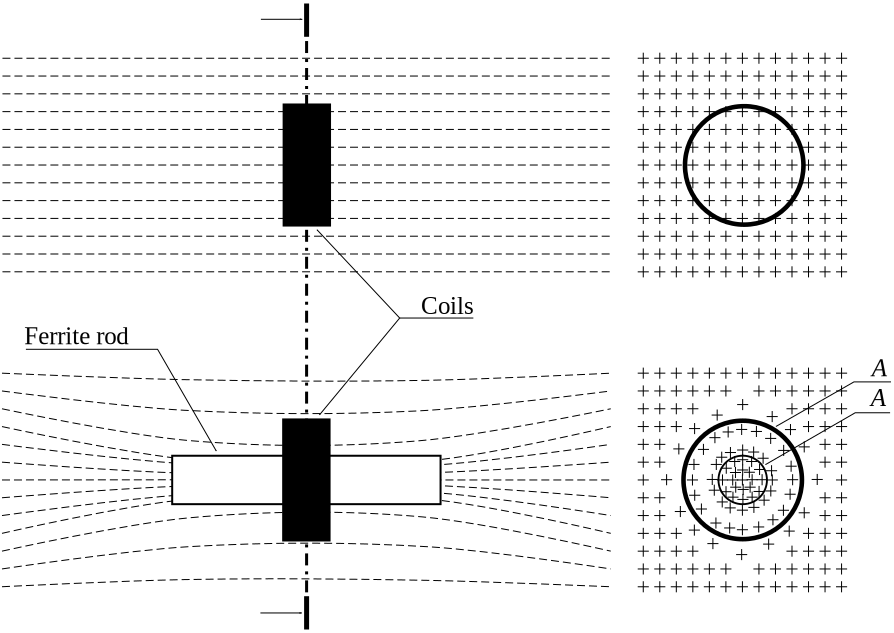
\includegraphics[width=11cm]{ch2/img/flux_lines.pdf}
	\begin{tikzpicture}[auto,>=latex]
		%\draw[style=help lines] (-3,-3) grid (9,3);
		\foreach \y in {1,...,9} {
			\draw[color=gray,dashed] (-3,0.3*\y+0.3) -- (3,0.3*\y+0.3); 
			\draw[color=gray,dashed] (-3,-0.3*\y) .. controls (0,-0.1*\y-1) .. (3,-0.3*\y); 
		}
		\coordinate (center2) at (0,-1.5);
		\coordinate (center1) at (0,3-4*0.3);
		
		\draw [dashdotted] (0,3.75) -- (0,-3.75);
		\draw [line width=2] (0,3.25) -- (0,3.75);
		\draw [line width=2] (0,-3.25) -- (0,-3.75);
		\draw [->] (-0.75,-3.5) -- (0,-3.5);
		\draw [->] (-0.75,3.5) -- (0,3.5);


		\draw [fill=white] ($ (center2) + (-1.5,0.25) $) -- ++(3,0) -- ++(0,-0.5) -- ++(-3,0) -- cycle;
		\draw [fill=black] ($ (center1) + (-0.25,0.5) $) -- ++(0.5,0) -- ++(0,-1) -- ++(-0.5,0) -- cycle;
		\draw [fill=black] ($ (center2) + (-0.25,0.5) $) -- ++(0.5,0) -- ++(0,-1) -- ++(-0.5,0) -- cycle;
		
		\coordinate (rcenter1) at ($ (center1) + (5,0) $);
		\coordinate (rcenter2) at ($ (center2) + (5,0) $);

		\foreach \y in {0,...,18} {
		\foreach \x in {1,...,5} {
			\node [circle,draw=gray,inner sep=0.5pt, fill=gray,at=(rcenter1.0),shift=(20*\y:\x*0.25)] {};
		}}

		\foreach \y in {0,...,18} {
		\foreach \x in {1,...,15} {
			\node [circle,draw=gray,inner sep=0.5pt, fill=gray,at=(rcenter2.0),shift=(20*\y:0.00035*\x*\x*\x)] {};
		}}

		\draw[fill=white] (rcenter2) circle (0.25);
		\draw [line width=1.3](rcenter2) circle (0.5);
		\draw [line width=1.3](rcenter1) circle (0.5);

		\draw [<-] ($ (rcenter2) + (50:0.25) $) -- ++(50:1.3) -- ++(1,0) node[above,pos=0.6]{$A_r$};
		\draw [<-] ($ (rcenter1) + (50:0.5) $) -- ++(50:1) -- ++(1,0) node[above,pos=0.6]{$A$};

		\draw [<-] ($ (center1) + (65:0.65) $) -- ++(50:1) -- ++(1,0) node[above,pos=0.6]{Coil};
		\draw [<-] ($ (center2) + (1,0) + (65:0.35) $) -- ++(50:1.25) -- ++(2,0) node[above,pos=0.6]{Ferrite rod};
			
	\end{tikzpicture}
	\label{fig:flussoferrite}
	\caption{Flux lines through coil and ferrite rod}
	\forceversofloat
\end{figure}
\arraymath{
	\Phi_T & = & \Phi_{\bfield_1} + \Phi_{\bfield_2} \\
	\Phi_{\bfield_1} & = & \magperm_r A_r H \\
	\Phi_{\bfield_2} & = &\magperm_0 (A-A_r) H
}
and thus the total flux is:
\begin{equation}
\Phi_T = H A_r \braces{ \magperm_r + \magperm_0 \braces{ \dfrac{A}{A_r} - 1} }
\end{equation}
bringing the previous equation in \ref{eq:tensioneindotta}, and simplifying with respect to constant parts of area, we get:
\begin{equation}
\vind = \omegaarva \numerospire \dfrac{E}{c} A_r \braces{\magperm_r + \braces{\dfrac{\diameter_c^2}{\diameter_r^2}-1}}
\end{equation}
In a real coil, we have a coil diameter that is ${\diameter_c = \diameter_c' + \diameter_\mathrm{wire}}$, and it is usual to approximate ${\diameter_c \approx \diameter_r}$, and our antenna equation becomes:
\begin{equation}
\vind = \omegaarva \numerospire \dfrac{E}{c} A_r \magperm_r
\end{equation}
From which appears that the insertion of a ferrite rod in a coils inductance brings to an increase of induced tension proportional to the value of magnetic permeability of the ferrite itself. The identification of this value is not trivial and should be done experimentally. There are only some numerical approximation to the value of $\magperm_0$ related to the dimensions of ferrite bar, but it appears evidently a correlation between the ratio bar length/bar diameter. The greater this ratio, the greater the value of permeability\sidenote{We could give a trivial interpretation to this statement: the greater the length of the ferrite bar, the greater the number of flux lines that are bended into the bar; also the smaller the diameter, the grater the density of bended flux lines, thus the greater the permeability value.}. 
\begin{equation}
\magperm_r \propto \dfrac{l_r}{\diameter_r}
\end{equation}

\myparagraph{Antenna effective height}
Effective height of antenna is defined as the ratio between the induced potential in the coils end the electric field intensity:
\begin{equation}
\altezzaeffettiva = \dfrac{\vind}{E}
\end{equation}
Applying previous equation to the definition of effective height:
\begin{equation}
\altezzaeffettiva = \dfrac{\omegaarva \numerospire A_r}{c} \braces{\magperm_r + \braces{\dfrac{\diameter_c^2}{\diameter_r^2}-1}}
\end{equation}

\subsection{Equivalent circuit and noise}
From a pure circuit point of view, ferrite antenna is seen as an an RLC circuit, in which we identify three passive components:
\begin{itemize}
\item $L\rightarrow\mathbf{Z}_L = j\omega L$: coil inductance
\item $R_p\rightarrow\mathbf{Z}_R = R_p$: wire resistance
\item $C\rightarrow\mathbf{Z}_C = (j\omega L)^{-1}$: parassite capacitance
\end{itemize}
The input voltage of the circuit is $\vind=\altezzaeffettiva E$
\begin{marginfigure}
	\centering
	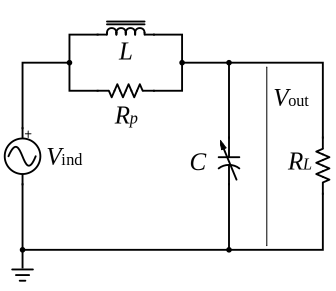
\includegraphics[width=5cm]{ch2/img/circuito_eq.pdf}
	\caption{Antenna equivalent circuit}
\end{marginfigure}

\myparagraph{Signal}
Starting from the definition of the equivalent circuit, with an external resistive load $R_L$ it is possible to derive a transfer function (full derivation in appendix at equation \ref{eq:transferfunc}):
\begin{equation}
\dfrac{V_{\mathrm{out}}}{\vind} = G(s) = \dfrac{\omega_{LC}}{Q_{\alpha}} \dfrac{s + Q_{\alpha} \omega_{LC}}{s^2 + \dfrac{\omega_{LC}}{Q_{\beta}} s + \omega_{LC}^2}
\end{equation}
\marginnote{\arraymath{
	\omega_{LC}^2 & = & \dfrac{1}{LC} \\
	Q_{\alpha} & = & \omega_{LC} R_P C \\
	Q_{\beta} & = & \omega_{LC} \dfrac{R_P R_L}{R_P + R_L} C
}}
if we obtain an ${\omega_{LC} = \omegaarva}$, we get resonance for an ARTVA incident signal: ${s=j\omegaarva}$:
\begin{equation}
G(j\omegaarva) = \left( -j Q_{\beta} \right) \left( 1 + \dfrac{j}{Q_{\alpha}} \right)
\end{equation} 
and then:
\begin{equation}
V_{\mathrm{out}} = \altezzaeffettiva \dfrac{Q_{\beta}}{Q_{\alpha}} E
\end{equation}

\myparagraph{Noise}
We could consider different sources of noise for our ferrite antenna:
\begin{itemize}
\item Boltzmann temperature noise
\item ferrite polarization noise
\item skin effect noise
\item auto-inductance noise
\item parasite capacitances due to construction, wirings or circuit grounding
\end{itemize}

Even if some of those source are easily to model, some of them are not and require an experimental interpolation. For the Boltzmann withe noise:
\[
V_{n,B} = \sqrt{4 \boltzmann T \Delta f Q_{\beta} \mathbf{Z}_{L}}
\]
that is environment dependent. For the other sources, some more considerations must be derived. Skin effect and ferrite noise are proportional to the received field. 
Those two effects must be carefully taken into account and analyzed from experimental point of view. The first one is due to the distribution of the current in the section of the coil wire: current tends to accumulate in the skin layer of the wire, generating eddy currents that are sources of noise. To this effect, some special woven wire, like litz wire, should be used.
The second effect, ferrite noise, derives from the polarization of the magnetic crystal inside ferrite. To polarize the whole ferrite bar, some energy must be spent to move magnetic domain, and the movement of those domain generates a noise. This effect is strictly related to the quality of material and cannot be mitigated.
Auto-inductance noise is due to the current that is absorbed by the serial circuit of antenna and load. In a production of a prototype it is important that input of identification circuit has a very high impedance to reduce a generation of this current on antenna. Some high quality devices implement a secondary loop on the antenna that acts as a re-generator, that tries to null those parasitic currents effect.

It is straightforward now, that all those noise effect could be resumed in an unique interpolated expression ${n \braces{\vind,T}}$.

For simulation purpose it is possible to simulate this as Gaussian white noise as follows:
\begin{equation}
\sigma = N\braces{\mathbf{0}, V_{n,B}} + 10^{x} \abs{\vind} N\braces{\mathbf{0}, \Sigma}
\end{equation}
with $x$ a value that scales the proportional noise.